\documentclass[article, 10pt]{disser}
\usepackage[a4paper,
            mag=1000, includefoot,
            left=3cm, right=1.5cm, top=2cm, bottom=2cm, headsep=1cm, footskip=1cm]{geometry}
\usepackage[T2A]{fontenc}
\usepackage[utf8]{inputenc}
\usepackage[english, russian]{babel}
\ifpdf\usepackage{epstopdf}\fi
\pagestyle{plain}
\usepackage{mathtext}
\usepackage{amsmath}
\usepackage{amsthm}
\usepackage{amsfonts}
\usepackage{float}
\usepackage{multirow}
\usepackage[usenames]{color}
\usepackage{listings}
\usepackage{colortbl}
\usepackage[unicode, pdftex]{hyperref}
\usepackage{amssymb}
\usepackage{graphicx}
\usepackage{hyperref}
\usepackage{wrapfig}
\usepackage{subfiles}
\usepackage{physics}
\usepackage{bm}
\usepackage{xcolor}
\usepackage{color} 
\usepackage{listings}
\usepackage{caption}
\usepackage{algorithm}
\usepackage{algpseudocode}

\newtheorem{theorem}{Теорема}
\newtheorem{proposition}{Утверждение}
\newtheorem{definition}{Определение}
\newtheorem{remark}{Замечание}
\newtheorem{proving}{Доказательство}
\DeclareMathOperator{\diag}{diag}
\DeclareMathOperator*{\argmin}{arg\,min}

% Точка с запятой в качестве разделителя между номерами цитирований
%\setcitestyle{semicolon}

% Использовать полужирное начертание для векторов
\let\vec=\mathbf

% Включать подсекции в оглавление
\setcounter{tocdepth}{2}

\graphicspath{{fig/}}

%----------------------------------------------------------------
\begin{document}

\topic{Обучение без учителя. Разделение смеси распределений. Кластеризация. Тематическое обучение (Probabilistic LSA).}
    

\city{Санкт-Петербург}
\date{\number\year}

\maketitle

\tableofcontents

\chapter{Кластерный анализ}
\section{Обучение без учителя}
Такие задачи как регрессионный анализ и классификация, являются задачами, которые предполагают так называемое обучение с учителем. В этом случае нам известны как независимые переменные $X_{1}, ... , X_{p},$ так и зависимая переменная $Y$. В случае обучения без учителя известны лишь $X_{1}, ... , X_{p}$. В таком случае мы не ставим задачу предсказания.

Проблема задач обучения без учителя заключается в том, что их сложно формализовать. И если в случае обучения с учителем есть явная оценка качества алгоритма, то для обучения без учителя её может и не быть, поэтому приходится использовать эвристические подходы для суждений о качестве результатов.
С помощью обучения без учителя можно решать такие задачи как:

\begin{itemize}

\item Кластеризация (иерархическая кластеризация, k-means). Задача состоит в том, чтобы предоставить исследователю алгоритм для разделения объектов на классы на основании их сходства.

\item Сокращение размерности (PCA). Если число признаков достаточно большое, то можно поставить задачу представления этих данных в пространстве меньшей размерности, таким образом, чтобы при этом потеря информации была минимальной.

\item Визуализация данных. Так как у нас есть возможность представить данные в пространстве размерности два, можно изобразить многомерные данные на плоскости, такой способ визуализации данных может быть полезным для их дальнейшего анализа.

\end{itemize}


\section{Кластеризация}

Задача кластеризации заключается в том чтобы выполнить разбиение индивидов на кластеры на основе их сходства друг с другом (близость относительно выбранной метрики), при этом сами кластеры или их количество, как правило, заранее не известны. Кластеры строятся так, что характеристики для объектов внутри одного кластера близки, а характеристик объектов из разных кластеров сильно отличаются. 

Пусть $C$ --- множество кластеров, $X$ --- пространство объектов, обучающая выборка это набор $X^{N}  = \{X_{i}\}_{i = 1}^{N} \subset X$, где $X_{i} \in \mathrm{R^{p}}$ --- это индивиды определяемые вектором признаков. Задача состоит в том чтобы найти такую функцию $a: X \rightarrow Y$, которая разбила бы выборку на непересекающиеся кластеры $X^{N} = \bigcup_{j = 1}^{k} C_{j}, \  C_{i} \bigcap C_{j} = \emptyset$, таким образом, чтобы объекты одного кластера были близки по функции расстояния между объектами $\rho : X \times X \rightarrow [0,\infty)$ и существенно отличались для объектов разных кластеров.

Общая схема процесса кластеризации данных включает пять основных этапов: 

\begin{itemize}

\item определение меры сходства;

\item разбиение множества объектов на кластеры;

\item оценка качества кластеризации;

\item выделение существенных характеристик исследуемых объектов;

\item интерпретация результатов.

\end{itemize}

Не существует <<истинных>> или <<лучших>> определений для кластера. Что понимать под кластером должно быть определено исследователем, который применяет методы кластеризации. Как правило, для этого нужно определить характеристики кластера в отношении размера и формы, а также предполагаемых различий между кластерами. На рисунке ниже (Рис.1)\footnote{https://github.com/NSHipster/DBSCAN} изображены различные формы кластеров (концентрические, ленточные, с гауссовским распределением). На последнем изображении показаны данные без кластерной структуры.

\begin{figure}[H]
\begin{center}
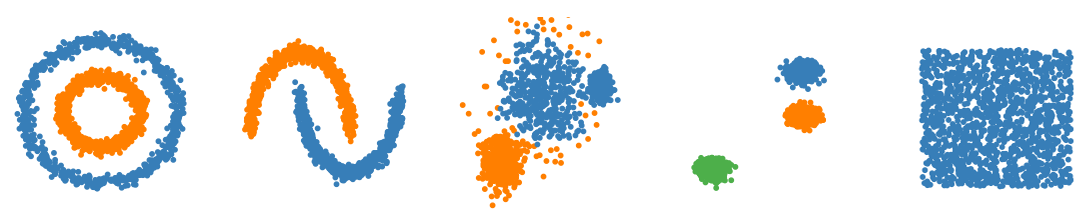
\includegraphics[scale = 0.3]{shape.png}
\caption{Различные формы кластеров}
\end{center}
\end{figure}

\subsection{EM - алгоритм}

Один из вариантов формализовать задачу кластеризации это сделать предположение о статистическом распределении данных. Затем задача будет состоять в поиске параметров этого распределения. Предположим, что модель данных состоит из $k$ смеси распределений. Пусть $\omega_{1}\ldots \omega_{k}$ --- априорные вероятности появления объектов из соответствующих кластеров, $p_{1}(x)\ldots p_{k}(x)$ --- плотности распределения признаков внутри кластеров. Тогда плотность распределения сразу для всех кластеров равна взвешенной сумме плотностей по каждому кластеру:
\begin{equation}
p(x) = \sum\limits_{i=1}^k \omega_{i} p_{i}(x).
\end{equation}
Поставим задачу разделения смеси распределений, оценим по выборке $\omega_{1}\ldots \omega_{k}$ и $p_{1}(x)\ldots p_{k}(x)$. Это позволит оценить вероятность принадлежности индивида к разным кластерам и решить к какому кластеру его отнести. Часто рассматриваются случаи когда распределение смеси принадлежат одному семейству распределений, например нормальному, но с разным набором параметров для каждого из кластеров. 
\begin{equation}
p_{i}(x) = \varphi(\theta_{i}; x)
\end{equation}
Согласно методу максимального правдоподобия 
\begin{equation}\label{maxlog} 
\omega, \theta = \underset{\omega, \theta}{\text{argmax}} \sum\limits_{i=1}^n \ln{p(x_{i})}  =  \underset{\omega, \theta}{\text{argmax}} \sum\limits_{i=1}^n \ln  \sum\limits_{j=1}^k \omega_{j}  \varphi(\theta_{j}; x_{i})
\end{equation}
Максимизация логарифма суммы достаточно сложна, поэтому задача не решается напрямую с помощью метода максимума правдоподобия. Для максимизации логарифма функции правдоподобия применяется EM-алгоритм. Это итеративный алгоритм, состоящий из двух шагов, в котором на первом шаге задаются какие-нибудь значения параметров, а затем с каждой итерацией эти параметры уточняются.

\textbf{E - шаг.}

В начале работы алгоритма задаём значения параметров $\omega, \theta = (\omega_{1}\ldots, \omega_{k};\theta_{1}\ldots \theta_{k})$, и подставляя их рассчитываем скрытые переменные. Скрытые переменные $h_{ij} = P(\theta_{j}|x_{i})$ --- это вероятность того, что индивид $x_{i}$ принадлежит $j$ смеси. Найдем скрытые переменные по формуле Байеса:
\begin{equation}
h_{ij} = \frac{ \omega_{j} \varphi(\theta_{j}; x_{i})}{\sum\limits_{s=1}^k \omega_{s}  \varphi(\theta_{s}; x_{i})}.
\end{equation}
Для любого индивида $\sum\limits_{j=1}^k h_{ij} = 1.$

\textbf{M - шаг.}

На этом шаге будут рассчитываться значения параметров, которые мы ищем, используя скрытые параметры, полученные на предыдущем шаге. Решение методом Лагрнажа для максимизации (\ref{maxlog}) (c ограничением $\sum\limits_{j=1}^k\omega_{j}=~1$) даёт оценку для параметров:
\begin{equation}
\omega_{j} = \frac{1}{n} \sum\limits_{i=1}^n h_{ij}
\end{equation}
\begin{equation}
\theta_{j} = \underset{\theta}{\text{argmax}} \sum\limits_{i=1}^n h_{ij} \ln{\varphi(\theta; x_{i})}
\end{equation}
Таким образом, параметры будут уточняться на каждом шаге.

Если сделать предположение о том что классы принадлежат семейству нормальных распределений, то параметрами модели являются математическое ожидание и ковариационная матрица. Если не делать никаких предположений о ковариациях использование общей модели может быть весьма затруднительно, проблема заключается в большом количестве параметров, которые необходимо оценить. Ковариационные матрицы описывают геометрические характеристики кластеров, а именно объем, форму и ориентацию кластера. Общая модель предполагает, что все эти геометрические характеристики различны для каждого кластера. Однако, оценка плотности смеси, состоящей из кластеров одинаковой формы или ориентации, намного проще. Поэтому, сделав предположения о ковариационных матрицах, можно существенно облегчить задачу.

\subsection{Алгоритм k-средних (k-means)}
Далее обсудим один из самых популярных алгоритмов кластеризации --- алгоритм k-средних. Евклидово расстояние: 
\begin{equation}
d(x_{i}, x_{i'}) = \sum\limits_{j=1}^k (x_{ij} - x_{i'j})^{2} = \| x_{i} - x_{i'} \|^{2},
\end{equation}
выбрано в качестве меры близости. Хотим минимизировать меру близости между индивидами внутри одного кластера. Для этого решаем следующую задачу: 
\begin{equation}
\underset{C_{1},\ldots, C_{k}}{\text{minimize}} \left\{ \sum\limits_{l=1}^k \frac{1}{|C_{l}|}  \sum\limits_{i,i' \in C_{l}} \sum\limits_{j = 1}^{p} (x_{ij} - x_{i'j})^{2} \right\} 
\end{equation}
$$
\underset{C_{1},\ldots, C_{k}}{\text{minimize}} \left\{ \sum\limits_{l=1}^k \frac{1}{|C_{l}|} \sum\limits_{i,i' \in C_{l}}   \| x_{i} - x_{i'} \|^{2} \right\}
$$
Идея алгоритма следующая: инициализируем центры, затем разделяем индивиды по ближайшему центру кластера, перевычисляем каждый из центров, и если ничего не изменилось, останавливаемся, если изменилось, то повторяем.

\begin{algorithm}
\caption{Алгоритм k-средних}\label{alg:cap}
1. Выбираем $\mu_{1},\ldots, \mu_{k}$ --- центры кластеров случайным образом.

2. Определяем принадлежность индивидов кластерам. Относим индивиды к тому кластеру $C_{j}$ центр $\mu_{j}$ которого находится ближе центров остальных кластеров.  $$C(i) = \underset{0 \leq j \leq  k}{\text{argmin}} \|x_{i} - \mu_{j} \|^{2}.$$

3. Для каждого кластера $C_{j}$ пересчитываем центры $\mu_{j}$ как выборочное среднее индивидов, которые были отнесены к этому кластеру.

4. Повторяем шаги 2 и 3 пока принадлежность кластерам не перестанет изменяться.
\end{algorithm}
Проблема метода заключается в том, что он чувствителен к выбору начального приближения для центров. Неудачный выбор кластеров может привести к плохому результату кластеризации. Для решения этой проблемы можно провести кластеризацию с несколькими начальными приближениями и выбрать лучший вариант. Кроме того,  нужно знать количество кластеров, и если выбрать неправильное количество, кластеризация также может оказаться неудачной. Частично решить эту проблему можно построением кластеризации для разного количества кластеров и сравнением результатов. На (Рис.2) приведён пример применения алгоритма к кластерам разной формы.

\begin{figure}[H]
\begin{center}
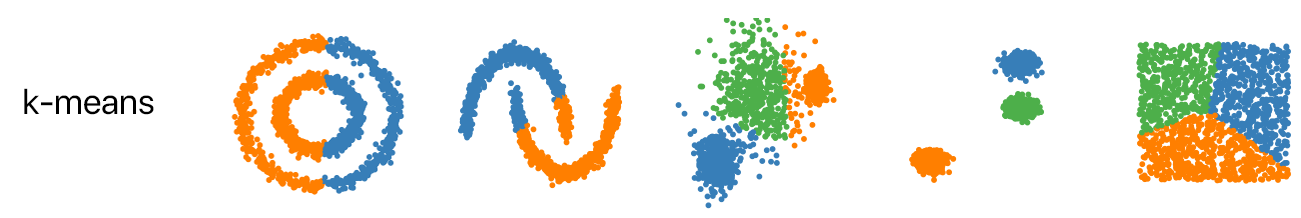
\includegraphics[scale = 0.25]{k - means.png}
\caption{k - means}
\end{center}
\end{figure}

Алгоритм k-средних тесно связан с EM-алгоритмом: он является частным случаем для гауссовой смеси распределения с диагональными матрицами, у которых все значения на диагонали равны. В таком случае, на Е-шаге мы не считаем вероятности принадлежности кластерам, а приписываем каждый объект одному кластеру (вероятность принадлежности будет равна 0 или 1). Кроме того, для этого частного случая форма кластеров не настраивается: они все являются сферическими.


\subsection{Иерархическая кластеризация}
Существует два типа иерархических кластеризаций: дивизионные и агломеративные. Первые начинают с одного кластера и разбивают его на множество более мелких кластеров, а вторые, наоборот, начинают с множества одноэлементных кластеров и на каждом шаге сливают наиболее близкие кластеры друг с другом. Более распространены агломеративные алгоритмы, общий вид которых приведён ниже. Результатом работы иерархического алгоритма является дендрограмма (график расстояний, при которых произошло слияние кластеров на каждом шаге).
\begin{center}
    \bf{Алгоритм иерархической кластеризации}
\end{center}
Дерево строится от листьев к корню. В начальный момент времени каждый объект содержится в собственном кластере. Далее происходит итеративный процесс слияния двух ближайших кластеров до тех пор, пока все кластеры не объединятся в один или не будет найдено необходимое число кластеров. На каждом шаге необходимо уметь вычислять расстояние между кластерами и пересчитывать расстояние между новыми кластерами. Расстояние между одноэлементными кластерами определяется через расстояние между объектами: $R(\{x\}, \{y\})= \rho(x,y)$. Для вычисления расстояния $R(U, V)$ между кластерами $U$ и $V$ на практике используются различные функции в зависимости от специфики задачи.

Главным вопросом в этом алгоритме является выбор расстояний между кластерами, поскольку от него сильно зависит результат кластеризации. Изначально было придумано множество различных способов определить такие расстояния, но оказалось, что практически все разумные, являются частным случаем формулы Ланса-Уильямса, приведённой ниже.\\
Формула Ланса-Уильямса:
\begin{equation*}
    R(W, S) = \alpha_{U}U R(U, S) + \alpha_{V} R(V, S) + \beta R(U, V) + \gamma|R(U, S) − R(V, S)|,
\end{equation*}
где $\alpha_{U}$, $\alpha_{V}$ , $\beta$, $\gamma$ --- числовые параметры.

Ниже приведены некоторые способы определения расстояний явно и соответствующие им коэффициенты для формулы Ланса-Уильямса.
\begin{itemize}
    \item Расстояние ближнего соседа:
    \begin{equation*}
        R(W, S) = \min\limits_{w\in W,s\in S}\rho(w, s);\quad\quad \alpha_U = \alpha_V = 1/2,\, \beta = 0,\, \gamma = −1/2;
    \end{equation*}
\item Расстояние дальнего соседа:
\begin{equation*}
R(W, S) = \max\limits_{w\in W,s\in S}\rho(w, s);\quad\quad \alpha_U = \alpha_V = 1/2,\, \beta = 0,\, \gamma = 1/2;
\end{equation*}
\item Среднее расстояние:
\begin{equation*}
R(W, S) = \frac{1}{|W||S|}\sum\limits_{w\in W}\sum\limits_{s\in S}\rho(w, s);\quad\quad \alpha_U = \frac{|U|}{|W|},\, \alpha_V = \frac{|V|}{|W||S|},\, \beta = \gamma = 0;
\end{equation*}
\item Расстояние между центрами:
\begin{equation*}
R(W, S) = \rho^{2}\left(\sum\limits_{w\in W}\frac{w}{|W|}, \sum\limits_{s\in S}\frac{s}{|S|}\right);\quad\quad \alpha_U = \frac{|U|}{|W|},\, \alpha_V = \frac{|V|}{|W||S|},\, \beta = -\alpha_{U}\alpha_{V},\, \gamma = 0;
\end{equation*}
\item Расстояние Уорда:
\begin{equation*}
R(W, S) = \frac{|S||W|}{|S|+|W|}\rho^{2}\left(\sum\limits_{w\in W}\frac{w}{|W|}, \sum\limits_{s\in S}\frac{s}{|S|}\right);
\end{equation*}
\begin{equation*}
\alpha_U = \frac{|S|+|U|}{|S|+|W|},\, \alpha_V = \frac{|S|+|V|}{|S|+|W|},\, \beta = -\frac{|S|}{|S|+|W|},\, \gamma = 0.
\end{equation*}
\end{itemize}

 Для визуального представления результатов кластеризации используется дендрограмма --- дерево, построенное по матрице мер близости между кластерами. В узлах дерева находятся подмножества объектов из обучающей выборки. При этом на каждом ярусе дерева множество объектов из всех узлов составляет исходное множество объектов. Объединение узлов между ярусами соответствует слиянию двух кластеров. При этом длина ребра соответствует расстоянию между кластерами. Введем обозначение $R_t$ --- расстояние между кластерами, выбранными на шаге $t$ для объединения. Дендрограмма позволяет представлять зависимости между множеством объектов с любым числом заданных характеристик на двумерном графике, где по одной из осей откладываются все объекты, а по другой --- расстояние $R_t$. Если не накладывать на это расстояние никаких ограничений, то дендрограмма будет иметь большое число самопересечений и изображение перестанет быть наглядным. Чтобы любой кластер мог быть представлен в виде непрерывного отрезка на оси объектов и ребра не пересекались, необходимо наложить ограничение монотонности на $R_t$.
 \begin{definition}
 Функция расстояния $R$ является монотонной, если на каждом следующем шаге расстояние между кластерами не уменьшается: $R_1 \leq R_2 \leq \dots \leq R_m$
 \end{definition}
Для определения числа кластеров находится интервал максимальной длины $|R_{t+1}−R_t|$. В качестве итоговых кластеров выдаются кластеры, полученные на шаге $t$. При этом число кластеров равно $m-t+1$. Однако, когда число кластеров заранее неизвестно и объектов в выборке не очень много, бывает полезно изучить дендрограмму целиком.

\section{Другие алгоритмы кластеризации}
\subsection{Алгоритм FOREL}
Алгоритм FOREL (ФОРмальный ЭЛемент) предложен Загоруйко и Ёлкиной в 1967 году при решении одной прикладной задачи в области палеонтологии. Алгоритм
имеет многочисленные вариации, в основе всех этих вариаций лежит следующая базовая процедура. Пусть задана некоторая точка $x_0 \in X$ и параметр $R$. Выделяются все точки выборки $x_i \in X^{l}$, попадающие внутрь сферы $\rho(x_i, x_0) \leq R$, и точка $x_0$ переносится в центр тяжести выделенных точек. Эта процедура повторяется до тех пор, пока состав выделенных точек, а значит и положение центра, не перестанет меняться. Доказано, что эта процедура сходится за конечное число шагов. При этом сфера перемещается в место локального сгущения точек. Центр сферы $x_0$ в общем случае не является объектом выборки, потому и называется формальным элементом. Для вычисления центра необходимо, чтобы множество объектов $X$ было не только метрическим, но и линейным векторным пространством. Это требование естественным образом выполняется, когда объекты описываются числовыми признаками. Однако существуют задачи, в которых изначально задана только метрика, а сложение и умножение на число не определены на $X$. Тогда в качестве центра сферы можно взять тот объект обучающей выборки, для которого среднее расстояние до других объектов кластера минимально. Соответственно, шаг 6 заменяется на
\begin{equation*}
    x_0 := \argmin\limits_{x \in K_0}\sum\limits_{x^{'}\in K_0}\rho(x, x^{'}).
\end{equation*}
\begin{enumerate}
       \item Пусть $U = X_m$
       \item \textbf{Пока} есть некластеризованные точки, т.е. $U \neq \varnothing$;
       \item \quadвзять случайную точку $x_0 \in U$;
       \item \quad\textbf{Повторять}
       \item \quad\quadобразовать кластер с центром в $x_0$ и радиусом $R$: $K_0 = \{x_i \in U |\, \rho(x_i, x_0) \leq R\}$;
       \item \quad\quadпереместить центр $x_0$ в центр масс кластера: $x_0 = \frac{1}{|K_0|}\sum\limits_{x_i \in K_0}x_i$;
       \item \quad\textbf{Пока} состав кластера K0 не стабилизируется;
       \item \quadПометить объекты внутри сферы как клаcтеризованные и  $U = U \backslash K_0$.
   \end{enumerate}

Алгоритм довольно чувствителен к выбору начального положения точки $x_0$ для каждого нового кластера. Для устранения этого недостатка предлагается генерировать несколько кластеризаций. Поскольку начальное положение центров выбирается случайным образом, эти кластеризации будут довольно сильно отличаться. Окончательно выбирается та кластеризация, которая доставляет наилучшее значение заданному функционалу качества.

\subsection{DBSCAN}
\textbf{DBSCAN} (Density-based spatial clustering of applications with noise) --- это эвристический алгоритм кластеризации, который предложили Маритин Эстер, Ганс-Петер Кригель, Ёрг Сандер и Сяовэй Су в 1996. Это алгоритм кластеризации, основанный на плотности --- алгоритм группирует вместе те объекты, которые тесно расположены, помечая как выбросы объекты, которые находятся в областях с малой плотностью.

В этом алгоритме рассматривается для каждого объекта $x \in U$ его $\epsilon$-окрестность $U_{\epsilon}(x) = \{u \in U : \rho(x, u) \leq \epsilon\}$. Каждый объект может быть одного из трёх типов:
\begin{itemize}
    \item корневой: имеет плотную окрестность $|U_{\epsilon}(x)| > m$
    \item граничный: не корневой, но находится в окрестности корневого
    \item выброс: не корневой и не граничный.
\end{itemize}
Корневые объекты находящиеся в $\epsilon$-окрестности друг друга объединяются в один кластер. Граничные объекты относятся к тому кластеру, к какому относится корневой объект, в $\epsilon$-окрестности которого лежит данный граничный объект. Таким образом, в итоге получается разделение всех объектов на кластеры и шумовые объекты. Более подробный алгоритм приведён ниже.

\begin{enumerate}
       \item $U = X_m,\; N = \varnothing,\; z = 0$;
       \item \textbf{Пока} есть некластеризованные точки, т.е. $U \neq \varnothing$;
       \item \quadвзять случайную точку $x \in U$;
       \item \quad\textbf{если} $|U_{\epsilon}(x)| < m$, \textbf{то}
       \item \quad\quad пометить $x$ как возможно шумовой;
       \item \quad\textbf{иначе}
       \item \quad\quad создать новый кластер: $K = U_{\epsilon}(x),\; z = z + 1$;
       \item \quad\quad\textbf{для всех} $x^{'} \in K$
       \item \quad\quad\quad\textbf{если} $|U_{\epsilon}(x^{'})| > m$ \textbf{то} $K = K \cup U_{\epsilon}(x^{'})$;
       \item \quad\quad\quad\textbf{иначе} пометить $x^{'}$ как граничный элемент $K$;
       \item \quad\quad$a(x_i) = z$ для всех $x^{'} \in K$;
       \item \quad\quad$U = U\backslash K$.
   \end{enumerate}
   
\begin{figure}
   \begin{center}
   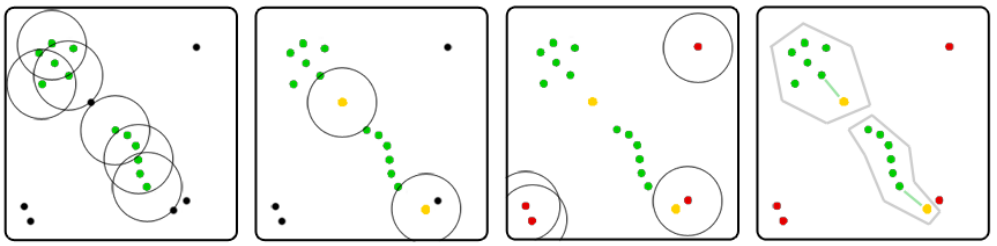
\includegraphics[scale = 0.4]{DBSCAN.png}
   \caption{Иллюстрация к алгоритму DBSCAN. На рисунке зелёным отмечены корневые объекты, жёлтым~---~граничные и красным~---~шумовые.}
   \end{center}
   \end{figure}
Алгоритм DBSCAN считается довольно быстрым (от $O(m \ln m)$ до $O(m^2)$ в зависимости от реализации) и позволяет обрабатывать кластеры произвольной формы. Помимо этого, DBSCAN выдаёт помимо деления на кластеры ещё и разметку шумовых объектов. Однако DBSCAN может плохо обрабатывать данные, в которых есть сильные вариации плотности внутри кластера, проёмы и шумовые мосты между кластерами.

\subsection{Самоорганизующаяся карта Кохонена}
Самоорганизующиеся карты Кохонена служат, в первую очередь, для визуализации и первоначального (<<разведывательного>>) анализа данных. Каждая точка данных отображается соответствующим кодовым вектором из решётки (далее в обозначениях $w_{mh}$). Так получают представление данных на плоскости (<<карту данных>>). На этой карте возможно отображение многих слоёв: количество данных, попадающих в узлы (то есть <<плотность данных>>), различные функции данных и так далее. При отображении этих слоёв полезен аппарат географических информационных систем (ГИС). В ГИС подложкой для изображения информационных слоев служит географическая карта. Карта данных является подложкой для произвольного по своей природе набора данных. Она служит заменой географической карте там, где ее просто не существует. Принципиальное отличие в следующем: на географической карте соседние объекты обладают близкими географическими координатами, на карте данных близкие объекты обладают близкими свойствами. С помощью карты данных можно визуализировать данные, одновременно нанося на подложку сопровождающую информацию (подписи, аннотации, атрибуты, информационные раскраски). Карта служит также информационной моделью данных. С её помощью можно заполнять пробелы в данных. Эта способность используется, например, для решения задач прогнозирования.

Чтобы продемонстрировать алгоритм введем следующие обозначения. По-прежнему $X$ --- пространство объектов, $\rho:\,X \times X$ --- метрика пространства объектов, $Y~=~\{1,\dots,M\} \times \{1,\dots,H\}$ --- сетка кластеров, $r: \, Y \times Y$ --- метрика пространства кластеров. Каждому узлу  $(m,h)$ сетки кластеров $Y$ приписан нейрон Кохонена $w_{mh}\in X$. Также заданы неотрицательные невозрастающие функции: $K(r(\cdot,\cdot),t)$ --- расстояние, $\eta(t)$ --- скорость обучения, $\epsilon(t)$ --- окрестность, где $t$ --- номер итерации, $\upsilon_{\epsilon(t)}(m_i,h_i)$ --- $\epsilon(t)$-окрестность $(m_i,h_i)$ в метрике $r$.
	\begin{figure}[H]
	\begin{center}
	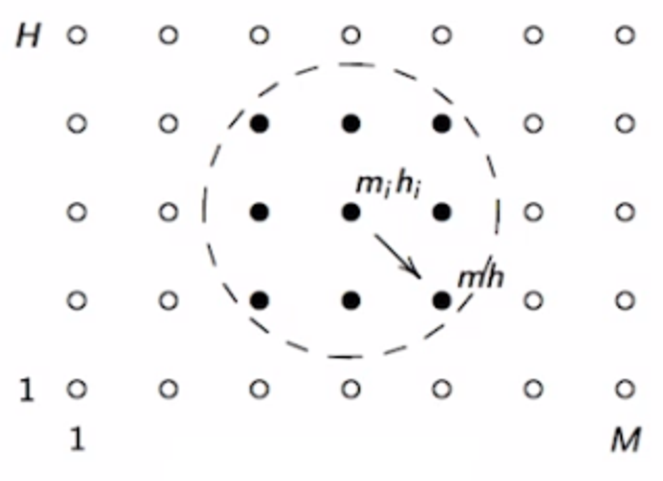
\includegraphics[width=0.4\textwidth]{karta.pdf}
	\caption{Решетка узлов карты}
	\end{center}
	\end{figure}
\noindent\textbf{Алгоритм обучения:}
	\begin{enumerate}
	\item задать начальные $w_{mh}$, $m=\overline{1:M}$, $h=\overline{1:H}$;
	\item {\bfповторять}
	\item\quad выбрать случайным образом $x_i$ из $X^n$;
	\item\quad вычислить координаты ближайшего кластера:
	$$(m_i,h_i)=\argmin_{(m,h)\in Y}\rho(x_i,w_{mh});$$
	\item\quad {\bfдля всех} $(m,h)\in\upsilon_{\epsilon}(m_i,h_i)$
	\item\qquad сделать шаг стохастического градиентного спуска:\\
	$\qquad w_{mh}=w_{mh}+\eta(t)(x_i-w_{mh})K\left(r[ (m_i,h_i),(m,h) ], t\right);$
	\item {\bfпока} кластеризация не стабилизируется;
	\end{enumerate}
	
Приведем особенности самоорганизующихся карт Кохонена (Self-Organising Maps, SOM). Устойчивость к зашумленным данным, возможность упрощения многомерных входных данных с помощью визуализации. SOM могут быть использованы для кластерного анализа только в том случае, если заранее известно число кластеров. Важным недостатком является то, что окончательный результат работы нейронных сетей зависит от начальных установок сети. С другой стороны, нейронные сети теоретически могут аппроксимировать любую непрерывную функцию, что позволяет исследователю не принимать заранее какие-либо гипотезы относительно модели.

\section{Функционалы качества кластеризации}
Задачу кластеризации можно ставить как задачу дискретной оптимизации: необходимо так приписать номера кластеров $y_i$ объектам $x_i$, чтобы значение выбранного функционала качества приняло наилучшее значение. Существует много разновидностей функционалов качества кластеризации, но нет <<самого правильного>> функционала. По сути дела, каждый метод кластеризации можно рассматривать как точный или приближённый алгоритм поиска оптимума некоторого функционала.

Среднее внутрикластерное расстояние должно быть как можно меньше:
\begin{equation*}
    F_0 = \frac{\sum_{i < j}\mathbf{I}_{\{y_i = y_j\}}\rho(x_i, x_j)}{\sum_{i < j}\mathbf{I}_{\{y_i = y_j\}}} \rightarrow \min.
\end{equation*}

Среднее межкластерное расстояние должно быть как можно больше:
\begin{equation*}
    F_1 = \frac{\sum_{i < j}\mathbf{I}_{\{y_i \neq y_j\}}\rho(x_i, x_j)}{\sum_{i < j}\mathbf{I}_{\{y_i \neq y_j\}}} \rightarrow \max.
\end{equation*}

Если алгоритм кластеризации вычисляет центры кластеров $\mu_y, y \in Y$, то можно определить функционалы, вычислительно более эффективные.

Сумма средних внутрикластерных расстояний должна быть как можно меньше:
\begin{equation*}
    \Phi_0 =  \sum\limits_{y \in Y}\frac{1}{|K_y|}\sum\limits_{i:\,y_i=y}\rho^2(x_i, \mu_y)\rightarrow \min,
\end{equation*}
где $K_y = \{x_i \in X^{n}| y_i = y\}$ --- кластер с номером $y$. В этой формуле можно было бы взять не квадраты расстояний, а сами расстояния. Однако, если $\rho$ евклидова метрика, то внутренняя сумма в $\Phi_0$ приобретает физический смысл момента инерции кластера $K_y$ относительно его центра масс, если рассматривать кластер как материальное тело, состоящее из $|K_y|$ точек одинаковой массы.

Сумма межкластерных расстояний должна быть как можно больше:
\begin{equation*}
    \Phi_1 =  \sum\lidmits_{y \in Y}\rho^2(\mu_y, \mu)\rightarrow \max,
\end{equation*}
где $\mu$ --- центр масс всей выборки.

На практике вычисляют отношение пары функционалов, чтобы учесть как межкластерные, так и внутрикластерные расстояния:
\begin{equation*}
    \frac{F_0}{F_1} \rightarrow \min,\quad \text{либо}\quad \frac{\Phi_0}{\Phi_1} \rightarrow \min.
\end{equation*}

Существует ещё множество различных более сложных функционалов качества. Смысл всех таких функционалов один и тот же: попытаться описать близость в кластерах и дальность между ними. Один из функционалов Силуэт строится следующим образом. Определяется принадлежность объекта своему кластеру как среднее расстояние от выбранного объекта до всех остальных объектов в его кластере
\begin{equation*}
    c(x_i) = \frac{1}{|K_i| - 1}\sum\limits_{x_j \in K_i,\, i\neq j}\rho(x_i, x_j)
\end{equation*}
и определяется принадлежность объекта другому кластеру, как среднее расстояние до всех объектов ближайшего чужого кластера
\begin{equation*}
    b(x_i) = \min\limits_{i\neq j}\frac{1}{|K_j|}\sum\limits_{x_z \in K_j}\rho(x_i, x_z)
\end{equation*}
Cилуэт такого объекта тогда равен
\begin{equation*}
    s(x_i) = \frac{b(x_i) - c(x_i)}{\max\{c(x_i), b(x_i)\}},
\end{equation*}
если $|K_i| > 1$ и $s(x_i) = 0$, если $|K_i| = 1$.

Значения силуэта изменяются от $-1$ до $1$, и кластеризация удалась лучше, если значение силуэта больше. Обычно, желательно, чтобы значение силуэта для кластеризации оказалось не менее $0.75$. Как видно из определения, для вычисления силуэта необходимо, чтобы кластеров было как минимум два. Ещё одна проблема его в том, что он не очень корректно обрабатывает ленточные кластеры, перекрывающиеся и кластеры с перемычками. Как только расстояние между объектами одного кластера становится сравнимым с расстоянием между объектами разных кластеров, силуэт перестаёт быть адекватным функционалом качества. Кроме того, в силуэт никак не заложен шум. Это значит, что если в данных встретится выброс, то силуэт будет больше (а значит, согласно ему, кластеризация удалась лучше), если выброс будет посчитан как отдельный кластер. Таким образом, данный функционал качества заточен именно под кластеры такого вида, когда они представляют собой далеко отстоящие компактные скопления объектов.

\chapter{Тематическое моделирование}
Тематическое моделирование (topic modeling) — одно из современных приложений машинного обучения к анализу текстов. Тематическая модель коллекции текстовых документов определяет, к каким темам относится каждый документ и какие слова (термины) образуют
каждую тему.

Вероятностная тематическая модель (ВТМ) описывает каждую тему дискретным распределением на множестве терминов, каждый документ - дискретным
распределением на множестве тем. Предполагается, что коллекция документов --- это последовательность терминов, выбранных случайно и независимо из смеси таких распределений, и ставится задача восстановления компонент смеси по выборке.

Поскольку документ или термин может относиться одновременно ко многим темам с различными вероятностями, говорят, что ВТМ осуществляет «мягкую» кластеризацию документов и терминов по кластерам-темам. Тем самым решаются проблемы синонимии и омонимии терминов, возникающие при обычной «жёсткой» кластеризации. Синонимы, часто употребляющиеся в схожих контекстах, с большой вероятностью попадают в одну тему. Омонимы, употребляющиеся в разных контекстах, распределяются между несколькими темами соответственно частоте употребления.

Некоторые приложения тематического моделирования:
\begin{itemize}
    \item разведочный поиск в электронных библиотеках;
    \item поиск тематического контента в соцсетях;
    \item детектирование и трекинг новостных сюжетов;
    \item мультимодальный поиск текстов и изображений;
    \item анализ банковских транзакционных данных;
    \item управление диалогом в разговорном интеллекте
\end{itemize}

\section{Model-based подход}
\subsection{Вероятностная модель коллекции документов}
Пусть $D$ --- множество (коллекция) текстовых документов, $W$ --- множество (словарь) всех употребляемых в них терминов (слов или словосочетаний). Каждый документ $d \in D$ представляет собой последовательность $n_d$ терминов $(w1, \dots, w_{n_d}$) из словаря $W$. Термин может повторяться в документе много раз.

\subsection{Постановка задачи}
Построить тематическую модель коллекции документов $D$ --- значит найти множество тем $T$, распределения $p(w |t)$ для всех тем $t \in T$ и распределения $p(t| d)$ для всех документов $d \in D$. Можно также говорить о задаче совместной <<мягкой>> кластеризации множества документов и множества слов по множеству кластеров-тем. Мягкая кластеризация означает, что каждый документ или термин не жёстко приписывается какой-то одной теме, а распределяется по нескольким темам.

Найденные распределения используются затем для решения прикладных задач.
Распределение $p(t| d)$ является удобным признаковым описанием документа в задачах информационного поиска, классификации и категоризации документов.

\subsection{Вероятностное пространство и гипотезы}
Предполагается, что существует конечное множество тем $T$, и каждое употребление термина $w$ в каждом документе $d$ связано с некоторой темой $t \in T$, которая не известна. Коллекция документов рассматривается как множество троек $(d, w, t)$, выбранных случайно и независимо из дискретного распределения $p(d, w, t)$, заданного на конечном множестве $D \times W \times T$. Документы $d \in D$ и термины $w \in W$ являются наблюдаемыми переменными, тема $t \in T$ является латентной (скрытой) переменной.

\textbf{Гипотеза о независимости} элементов выборки эквивалентна предположению, что порядок терминов в документах не важен для выявления тематики, то есть тематику документа можно узнать даже после произвольной перестановки терминов, хотя для человека такой текст теряет смысл. Это предположение называют гипотезой <<мешка слов>> (bag of words). Порядок документов в коллекции также не имеет значения; это предположение называют гипотезой <<мешка документов>>. Приняв гипотезу <<мешка слов>>, можно перейти к более компактному представлению документа как подмножества $d \subset W$, в котором каждому элементу $w \in d$ поставлено в соответствие число $n_{dw}$ вхождений термина $w$ в документ $d$.

\textbf{Гипотеза условной независимости.} Будем полагать, что появление слов в документе $d$, относящихся к теме $t$, описывается общим для всей коллекции распределением $p(w |t)$ и не зависит от документа $d$. Это предположение, называемое гипотезой условной независимости, допускает три эквивалентных представления:
\begin{equation}
    p(w | d, t) = p(w |t);\\
    p(d |w, t) = p(d |t);\\
    p(d, w |t) = p(d |t)p(w |t).
\end{equation}

\textbf{Гипотеза разреженности.} Естественно предполагать, что каждый документ $d$ и каждый термин $w$ связан с небольшим числом тем $t$. В таком случае значительная часть вероятностей $p(t| d)$ и $p(w |t)$ должна обращаться в нуль. Если документ относится к большому числу тем (например, энциклопедия, журнал, сборник статей), то в задачах тематического поиска или классификации документов его имеет смысл разбивать на части, более однородные по тематике. Если термин относится к большому числу тем, то, скорее всего, это общеупотребительное слово (стоп-слово), бесполезное для определения тематики.

\subsection{Предварительная обработка текстовых документов}
\begin{itemize}
    \item \textbf{Лемматизация} --- это приведение каждого слова в документе к его нормальной форме. В русском языке нормальными формами считаются: для существительных — именительный падеж, единственное число; для прилагательных — именительный падеж, единственное число, мужской род; для глаголов, причастий, деепричастий --- глагол в инфинитиве. Разработка хорошего лемматизатора (lemmatizer) требует составления грамматического словаря со всеми формами слов, либо аккуратной формализации правил языка со всеми исключениями, что является трудоёмким проектом. Известные лемматизаторы совершенствуются постепенно. Их недостатком является неполнота словарей, особенно по части специальной терминологии и неологизмов, которые во многих приложениях как раз и представляют наибольший интерес.

\item \textbf{Стемминг} --- это более простая технология, которая состоит в отбрасывании изменяемых частей слов, главным образом, окончаний. Она не требует хранения словаря всех слов и основана на правилах морфологии языка. Недостатком стемминга является большее число ошибок. Стемминг хорошо подходит для английского языка, но хуже подходит для русского.

\item \textbf{Отбрасывание стоп-слов.} Слова, встречающиеся во многих текстах различной тематики, бесполезны для тематического моделирования, и могут быть отброшены. К ним относятся предлоги, союзы, числительные, местоимения, некоторые глаголы, прилагательные и наречия. Число таких слов обычно варьируется в пределах нескольких сотен. Их отбрасывание почти не влияет на длину словаря, но может приводить к заметному сокращению длины некоторых текстов.

\item \textbf{Отбрасывание редких слов.} Слова, встречающиеся в длинном документе слишком редко, например, только один раз, также можно отбрасывать, полагая, что данное слово не характеризует тематику данного документа. При обработке коллекций коротких новостных сообщений этот приём лучше не использовать.

\item \textbf{Выделение ключевых фраз.} При обработке коллекций научных, юридических или других специальных текстов вместо отдельных слов выделяют ключевые фразы --- словосочетания, являющиеся терминами предметной области. Это отдельная довольно сложная задача, для решения которой используются тезаурусы, составленные экспертами, либо методы машинного обучения, при этом для формирования обучающих выборок всё равно приходится привлекать экспертов.
\end{itemize}

Далее будем полагать, что словарь $W$ получен в результате предварительной обработки всех документов коллекции $D$ и может содержать как отдельные слова, так и ключевые фразы. Элементы словаря $w \in W$ будем называть <<терминами>>.

\subsection{Частотные оценки условных вероятностей}
Вероятности, связанные с наблюдаемыми переменными $d$ и $w$, можно оценивать по выборке как частоты:
\begin{equation*}
    \hat{p}(d, w) = \frac{n_{dw}}{n},\quad \hat{p}(d) = \frac{n_{d}}{n},\quad \hat{p}(w) = \frac{n_{w}}{n},\quad \hat{p}(w | d) = \frac{n_{dw}}{n_{d}} \text{, где}
\end{equation*}
\begin{itemize}
    \item $n_{dw}$ --- число вхождений термина $w$ в документ $d$;
    \item $n_d = \sum\limits_{w \in W}n_{dw}$ --- длина документа $d$ в терминах;
    \item $n_w = \sum\limits_{d \in D}n_{dw}$ --- число вхождений термина $w$ во все документы коллекции;
    \item $n = \sum\limits_{d \in D}\sum\limits_{w \in W}n_{dw}$ --- длина коллекции в терминах.
\end{itemize}

Вероятности, связанные со скрытой переменной $t$, также можно оценивать как частоты, если рассматривать коллекцию документов как выборку троек $(d,\; w,\; t)$:
\begin{equation*}
    \hat{p}(t) = \frac{n_{t}}{n},\quad \hat{p}(w |t) = \frac{n_{wt}}{n_t},\quad \hat{p}(t| d) = \frac{n_{dt}}{n_d},\quad \hat{p}(t| d, w) = \frac{n_{dwt}}{n_{dw}} \text{, где}
\end{equation*}
\begin{itemize}
    \item $n_{dwt}$ --- число троек, в которых термин w документа d связан с темой $t$;
    \item $n_{dt} = \sum\limits_{w \in W}n_{dwt}$ --- число троек, в которых термин документа $d$ связан с темой $t$;
    \item $n_{wt} = \sum\limits_{d \in D}n_{dwt}$ --- число троек, в которых термин w связан с темой $t$;
    \item $n_t = \sum\limits_{d \in D}\sum\limits_{w \in W}n_{dwt}$ --- число троек, связанных с темой t.
\end{itemize}

В пределе $n \rightarrow \infty$ частотные оценки $\hat{p}(\cdot)$, стремятся к соответствующим вероятностям $p(\cdot)$, согласно закону больших чисел. Частотная интерпретация даёт ясное понимание всех условных вероятностей, которые будут использоваться в дальнейшем.


\section{Вероятностный латентный семантический анализ PLSA}
\subsection{Стохастическое матричное разложение}
Если число тем $|T|$ много меньше числа документов $|D|$ и числа терминов $|W|$, то равенство (1.2) можно понимать как задачу
приближённого представления заданной матрицы частот
\begin{equation*}
    F = (\hat{p}_{wd})_{W \times D},\quad \hat{p}_{wd} = \hat{p}(w | d) = \frac{n_{dw}}{n_d},
\end{equation*}
в виде произведения $F \approx \Phi\Theta$ двух неизвестных матриц меньшего размера --- матрицы терминов тем $\Phi$ и матрицы тем документов $\Theta$:
\begin{equation*}
    \Phi = (\varphi_{wt})_{W \times T},\quad \varphi_{wt} = p(w |t);
\end{equation*}
\begin{equation*}
    \Theta = (\theta_{td})_{T \times D},\quad \theta_{td} = p(t| d).
\end{equation*}
Матрицы, столбцы которых неотрицательны и нормированы, следовательно, могут пониматься как дискретные распределения, называются стохастическими. Одно из наиболее известных представлений вида $F \approx \Phi\Theta$ строится из $|T|$ главных компонент сингулярного разложения матрицы $F$ и является решением задачи наименьших квадратов
\begin{equation*}
    \sum\limits_{d \in D}\sum\limits_{w \in W}\left(\hat{p}_{wd} - p(w | d)\right)^{2} = \sum\limits_{d \in D}\sum\limits_{w \in W}\left(\hat{p}_{wd} - \sum\limits_{t \in T}\varphi_{wt}\theta_{td}\right)^{2}= ||F - \Phi\Theta||^{2} \rightarrow  \min\limits_{\Phi,\,\Theta}.
\end{equation*}
Метод главных компонент не подходит для тематического моделирования, так как получаемые с его помощью матрицы $\Phi,\, \Theta$ в общем случае не являются стохастическими. Кроме того, квадратичная функция потерь плохо подходит для сравнения вероятностных распределений с <<тяжёлыми хвостами>>. В вероятностном тематическом моделировании вместо принципа наименьших квадратов используется принцип максимума правдоподобия.

\subsection{Принцип максимума правдоподобия}
Для оценки параметров $\Phi, \Theta$ тематической модели по коллекции документов $D$ будем максимизировать правдоподобие выборки:
\begin{equation*}
    L(D;\,\Phi,\,\Theta) = C \prod\limits_{i=1}^{n}p(d_i, w_i) = C \prod\limits_{d \in D}\prod\limits_{w \in W}p(d, w)^{n_{dw}} = \prod\limits_{d \in D}\prod\limits_{w \in W}p(w|d)^{n_{dw}}Cp(d)^{n_{dw}},
\end{equation*}
где $C$ --- нормировочный множитель, зависящий только от чисел $n_dw$. Отбросим множители $C$ и $p(d)$, не влияющие на положение точки максимума, подставим выражение для $p(w|d)$ и воспользуемся обозначениями $\theta_{td} = p(t| d)$, $\varphi_{wt} = p(w |t)$. Прологарифмируем $L(D;\, \Phi,\, \Theta)$, чтобы от произведения перейти к сумме. Получим задачу максимизации логарифма правдоподобия при ограничениях неотрицательности и нормированности столбцов матриц $\Phi$ и $\Theta$:
\begin{equation*}
\begin{cases}
   \mathcal{L}(\Phi,\,\Theta) = \sum\limits_{d \in D}\sum\limits_{w \in W}n_{dw}\ln \sum\limits_{t \in T}\varphi_{wt}\theta_{td} \rightarrow \max\limits_{\Phi,\,\Theta}\\
   \varphi_{wt} \geq 0,\;\sum\limits_{w\in W}\varphi_{wt} = 1\\
   \theta_{td}\geq 0,\; \sum\limits_{t\in T}\theta_{td} = 1.
\end{cases}
\end{equation*}
Для решения этой задачи используется EM-алгоритм.

\subsection{EM-алгоритм}
Для решения задачи в PLSA применяется итерационный процесс, в котором каждая итерация состоит из двух шагов --- Е (expectation) и М (maximization). Перед первой итерацией выбирается начальное приближение параметров $\varphi_{wt},\, \theta_{td}$.

На E-шаге по текущим значениям параметров $\varphi_{wt},\, \theta_{td}$ с помощью формулы Байеса вычисляются условные вероятности $p(t| d, w)$ всех тем $t \in T$ для каждого термина $w \in W$ в каждом документе $d$:
\begin{equation*}
   H_{dwt} = p(t| d, w) = \frac{p(w |t)p(t| d)}{p(w | d)} = \frac{\varphi_{wt}\theta_{td}}{\sum\limits_{s\in T}\varphi_{ws}\theta_{sd}}. 
\end{equation*}

На M-шаге, наоборот, по условным вероятностям тем $H_{dwt}$ вычисляется новое приближение параметров $\varphi_{wt},\, \theta_{td}$. Это легко сделать, если заметить, что величина 
\begin{equation*}
    \hat{n}_{dwt} = n_{dw}p(t| d, w) = n_{dw}H_{dwt}
\end{equation*}
оценивает (не обязательно целое) число $n_{dwt}$ вхождений термина $w$ в документ $d$, связанных с темой $t$. Просуммировав $\hat{n}_{dwt}$ по документам $d$ и по терминам $w$, получим оценки $\hat{n}_{wt}$, $\hat{n}_{dt}$, $\hat{n}_{t}$, и через них, согласно (1.4), --- частотные оценки условных вероятностей $\varphi_{wt},\, \theta_{td}$:
\begin{equation*}
    \varphi_{wt} = \frac{\hat{n}_{wt}}{\hat{n}_{t}},\quad \hat{n}_t =\sum\limits_{w \in W}\hat{n}_{wt},\quad \hat{n}_{wt} = \sum\limits_{d \in D}n_{dw}H_{dwt}.
\end{equation*}
\begin{equation*}
     \theta_{dt} = \frac{\hat{n}_{dt}}{\hat{n}_{t}},\quad \hat{n}_d =\sum\limits_{t \in T}\hat{n}_{dt},\quad \hat{n}_{dt} = \sum\limits_{w \in d}n_{dw}H_{dwt}.
\end{equation*}

Эти простые, но не вполне строгие рассуждения поясняют суть EM-алгоритма. Покажем теперь, что эти оценки действительно являются решением задачи максимизации правдоподобия при фиксированных $H_{dwt}$.

Запишем лагранжиан задачи при ограничениях нормировки, проигнорировав ограничения неотрицательности (позже убедимся, что решение действительно
неотрицательно):
\begin{equation*}
    \mathcal{L}(\Phi,\,\Theta) = \sum\limits_{d \in D}\sum\limits_{w \in W}n_{dw}\ln \sum\limits_{t \in T}\varphi_{wt}\theta_{td} - \sum\limits_{t \in T}\lambda_{t}\left(\sum\limits_{w \in W}\varphi_{wt}-1\right) - \sum\limits_{d \in D}\mu_d\left(\sum\limits_{t \in T}\theta_{td}-1\right).
\end{equation*}
Продифференцировав лагранжиан по $\phi_{wt}$ и приравняв нулю производную, получим
\begin{equation*}
    \lambda_t = \sum\limits_{d \in D}n_{dw}\frac{\theta_{td}}{p(w|d)}.
\end{equation*}
Домножим обе части этого равенства на $\varphi_{wt}$, просуммируем по всем терминам $w \in W$, применим условие нормировки вероятностей $\varphi_{wt}$ в левой части и выделим переменную $H_{dwt}$ в правой части. Получим
\begin{equation*}
    \lambda_t = \sum\limits_{d \in D}\sum\limits_{w \in W}n_{dw}H_{dwt}.
\end{equation*}
Снова домножим обе части на $\varphi_{wt}$, выделим переменную $H_{dwt}$ в правой части и выразим $\varphi_{wt}$ из левой части, подставив уже известное выражение для $\lambda_t$. Получим
\begin{equation*}
    \varphi_{wt} = \frac{\sum\limits_{d \in D}n_{dw}H_{dwt}}{\sum\limits_{d \in D}\sum\limits_{w^{'} \in W}n_{dw^{'}}H_{dw^{'}t}}
\end{equation*}

Обозначив числитель через $\hat{n}_{wt}$, получим (2.3). Проделав аналогичные действия с производной лагранжиана по $\theta_{td}$, получим (2.4). Заметим, что если начальные приближения $\theta_{td}$ и $\varphi_{wt}$ положительны, то и после каждой итерации они будут оставаться положительными, несмотря на то, что ограничение неотрицательности было проигнорировано в ходе решения.

Число операций алгоритма растёт линейно по длине коллекции $n$, числу тем $T$ и числу итераций. Перебор всех терминов $w$ во всех документах $d$ можно организовать очень эффективно, если хранить каждый документ $d$ в виде последовательности пар $(w, n_{dw})$.

Вычисление переменных $\hat{n}_{wt},\, \hat{n}_{dt},\, \hat{n}_t$ на М-шаге требует однократного прохода всей коллекции в цикле по всем документам $d \in D$ и всем терминам $w \in d$. Внутри этого цикла переменные $H_{dwt}$ можно вычислять непосредственно в тот момент, когда они понадобятся. От этого результат алгоритма не изменяется, Е-шаг встраивается внутрь M-шага без дополнительных вычислительных затрат, отпадает необходимость хранения трёхмерной матрицы $H_{dwt}$. Заметим также, что переменную $\hat{n}_d$ можно не вычислять, поскольку $\hat{n}_d=n_d$. Этот вариант реализации EM-алгоритма будем называть рациональным; он показан в Алгоритме 2.1.
\newpage
\begin{center}
    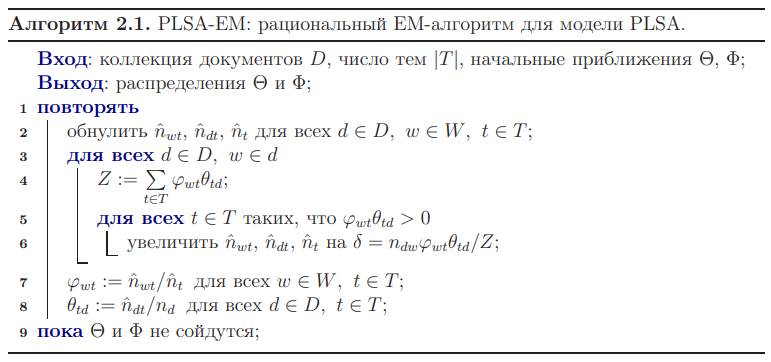
\includegraphics[scale = 0.75]{Em-алг.png}
\end{center}

\subsection{Начальное приближение}
Начальные приближения $\varphi_t$ и $\theta_d$ можно задавать нормированными случайными векторами из равномерного распределения.

Другая распространённая рекомендация --- пройти по всей коллекции, выбрать для каждой пары $(d, w)$ случайную тему $t$ и вычислить частотные оценки (1.4) вероятностей $\varphi_{wt}$ и $\theta_{td}$ для всех $d \in D$, $w \in W$, $t \in T$.

B случаях, когда темы известны заранее и имеются дополнительные данные о привязке некоторых документов или терминов к темам, применяется инициализация с частичным обучением. Учёт этих данных улучшает интерпретируемость тем.

Если известно, что документ $d$ относится к подмножеству тем $T_d \subset T$, то в качестве начального  $\theta_td$ можно взять равномерное распределение на этом подмножестве:
\begin{equation*}
    \theta_{td}^{0} = \frac{1}{|T_d|}\mathbf{I}_{t \in T_d}.
\end{equation*}
Если известно, что подмножество терминов $W_t \subset W$ относится к теме $t$, то в качестве начального $\varphi_wt$ можно взять равномерное распределение на $W_t$:
\begin{equation*}
   \varphi_{wt}^{0} = \frac{1}{|W_t|}\mathbf{I}_{w \in W_t}.
\end{equation*}

Если известно, что подмножество документов $D_t \subset D$ относится к теме $t$, то можно взять эмпирическое распределение слов в объединённом документе:
\begin{equation*}
   \varphi_{wt}^{0} = \frac{\sum_{d \in D_t}n_{dw}}{\sum_{d \in D_t}n_{d}}.
\end{equation*}

Если нет никакой априорной информации о связи документов с темами, то последнюю формулу можно применить к случайным подмножествам документов $D_t$.

\section{Критерии качества тематической модели}
В отличие от задач классификации или регрессии в оценке качества тематических моделей нет чёткого понятия <<ошибки>> или <<потери>>. Стандартные критерии качества кластеризации типа средних внутрикластерных или межкластерных расстояний или их отношений плохо подходят для оценивания <<мягкой>> совместной кластеризации документов и терминов.

Наиболее распространённым критерием является перплексия (perplexity), используемая для оценивания моделей языка в компьютерной лингвистике. Это мера
<<удивлённости>> модели $p(w | d)$ терминам $w$, наблюдаемым в документах $d$ коллекции $D$, определяемая через логарифм правдоподобия:
\begin{equation*}
    \mathcal{P}(D; p) = \exp\left(-\frac{1}{n}L(\Phi, \Theta)\right)= \exp \left( -\frac{1}{n}\sum\limits_{d \in D}\sum\limits_{w \in d}n_{dw}\ln p(w|d)\right).
\end{equation*}
Чем меньше эта величина, тем лучше модель $p$ предсказывает появление терминов $w$ в документах $d$ коллекции $D$.

Если термины $w$ порождаются из равномерного распределения $p(w) = 1/V$ на словаре мощности $V$, то перплексия модели $p$ на таком тексте сходится к $V$ с ростом его длины. Чем сильнее распределение $p$ отличается от равномерного, тем меньше перплексия. Чем сильнее модель $p$ отличается от генерирующего распределения, тем больше перплексия. В нашем случае используются условные вероятности терминов $p(w | d)$, и интерпретация немного другая: если каждый документ генерируется из $V$ равновероятных терминов (возможно, различных в разных документах), то перплексия сходится к $V$. Опять-таки, чем сильнее распределение отличается от равномерного, тем меньше перплексия.

Перплексия контрольной выборки. Обозначим через $p_D(w | d)$ модель, построенную по обучающей коллекции документов $D$. Перплексия обучающей выборки $\mathcal{P}(D; p_D)$ является заниженной характеристикой качества модели из-за эффекта переобучения. Обобщающую способность модели принято оценивать перплексией контрольной выборки (hold-out perplexity) $\mathcal{P}(D^{'}; p_D)$.

Вопрос о том, как разделить исходную коллекцию на обучение $D$ и контроль $D^{′}$, не тривиален. После обучения модели $p_D$ векторы $\phi_t$ фиксируются, векторы $\theta_d$ контрольных документов $d \in D^{′}$ оцениваются по первой половине каждого документа, по вторым половинам вычисляется контрольная перплексия. Что такое <<половина>>, не уточняется. Простое разрезание текста на две части может приводить к смещённым оценкам. Например, научные статьи обычно начинаются с введения и обзора, использующих общую терминологию, затем идёт изложение частных результатов. Если в коллекции много таких текстов, то оценка окажется пессимистично смещённой. Противоположный пример неслучайного разбиения текста --- когда число вхождений каждого термина $n_{dw}$ делится ровно пополам между обучающей и контрольной выборками. В таком случае обучающая и контрольная половины документа будут неразличимы для тематической модели, и оценка окажется оптимистично смещённой.

\textbf{Интерпретируемость тем.} Тема называется когерентной, если термины, наиболее частые в данной теме, неслучайно часто совместно встречаются рядом в документах коллекции. Когерентность может оцениваться по сторонней коллекции (например, по Википедии), либо по той же коллекции, по которой строится модель.

Предлагалось несколько оценок когерентности. Сначала использовалась поточечная взаимная информация (pointwise mutual information, PMI):
\begin{equation*}
    \text{PMI}(t) = \sum\limits_{i=1}^{k-1}\sum\limits_{j =i}^{k}\log\frac{N(w_i,\,w_j)}{N(w_i)N(w_j)},
\end{equation*}
где $w_i$ --- $i$-й термин в порядке убывания $\varphi_{wt}$, $N(w)$ --- число документов, в которых термин $w$ встречается хотя бы один раз, $N(w, w^{'})$ --- число документов, в которых термины $w$, $w^{'}$ встречаются рядом хотя бы один раз, число $k$ обычно полагается равным $10$. <<Встречаются рядом>> означает --- в окне заданной ширины.

Затем в экспериментах было показано, что более адекватной мерой когерентности является логарифм условной вероятности (log conditional probability,
LCP), оценивающая вероятность менее частого слова при условии более частого:
\begin{equation*}
    \text{LSP}(t) = \sum\limits_{i=1}^{k-1}\sum\limits_{j =i}^{k}\log\frac{N(w_i,\,w_j)}{N(w_i)}.
\end{equation*}
\end{document}



